\chapter{Diagrama Stea/Fulg a Bazei de Date Depozit OLAP}
\label{sec:diagrama_stea}

\begin{figure}[H]
    \centering
    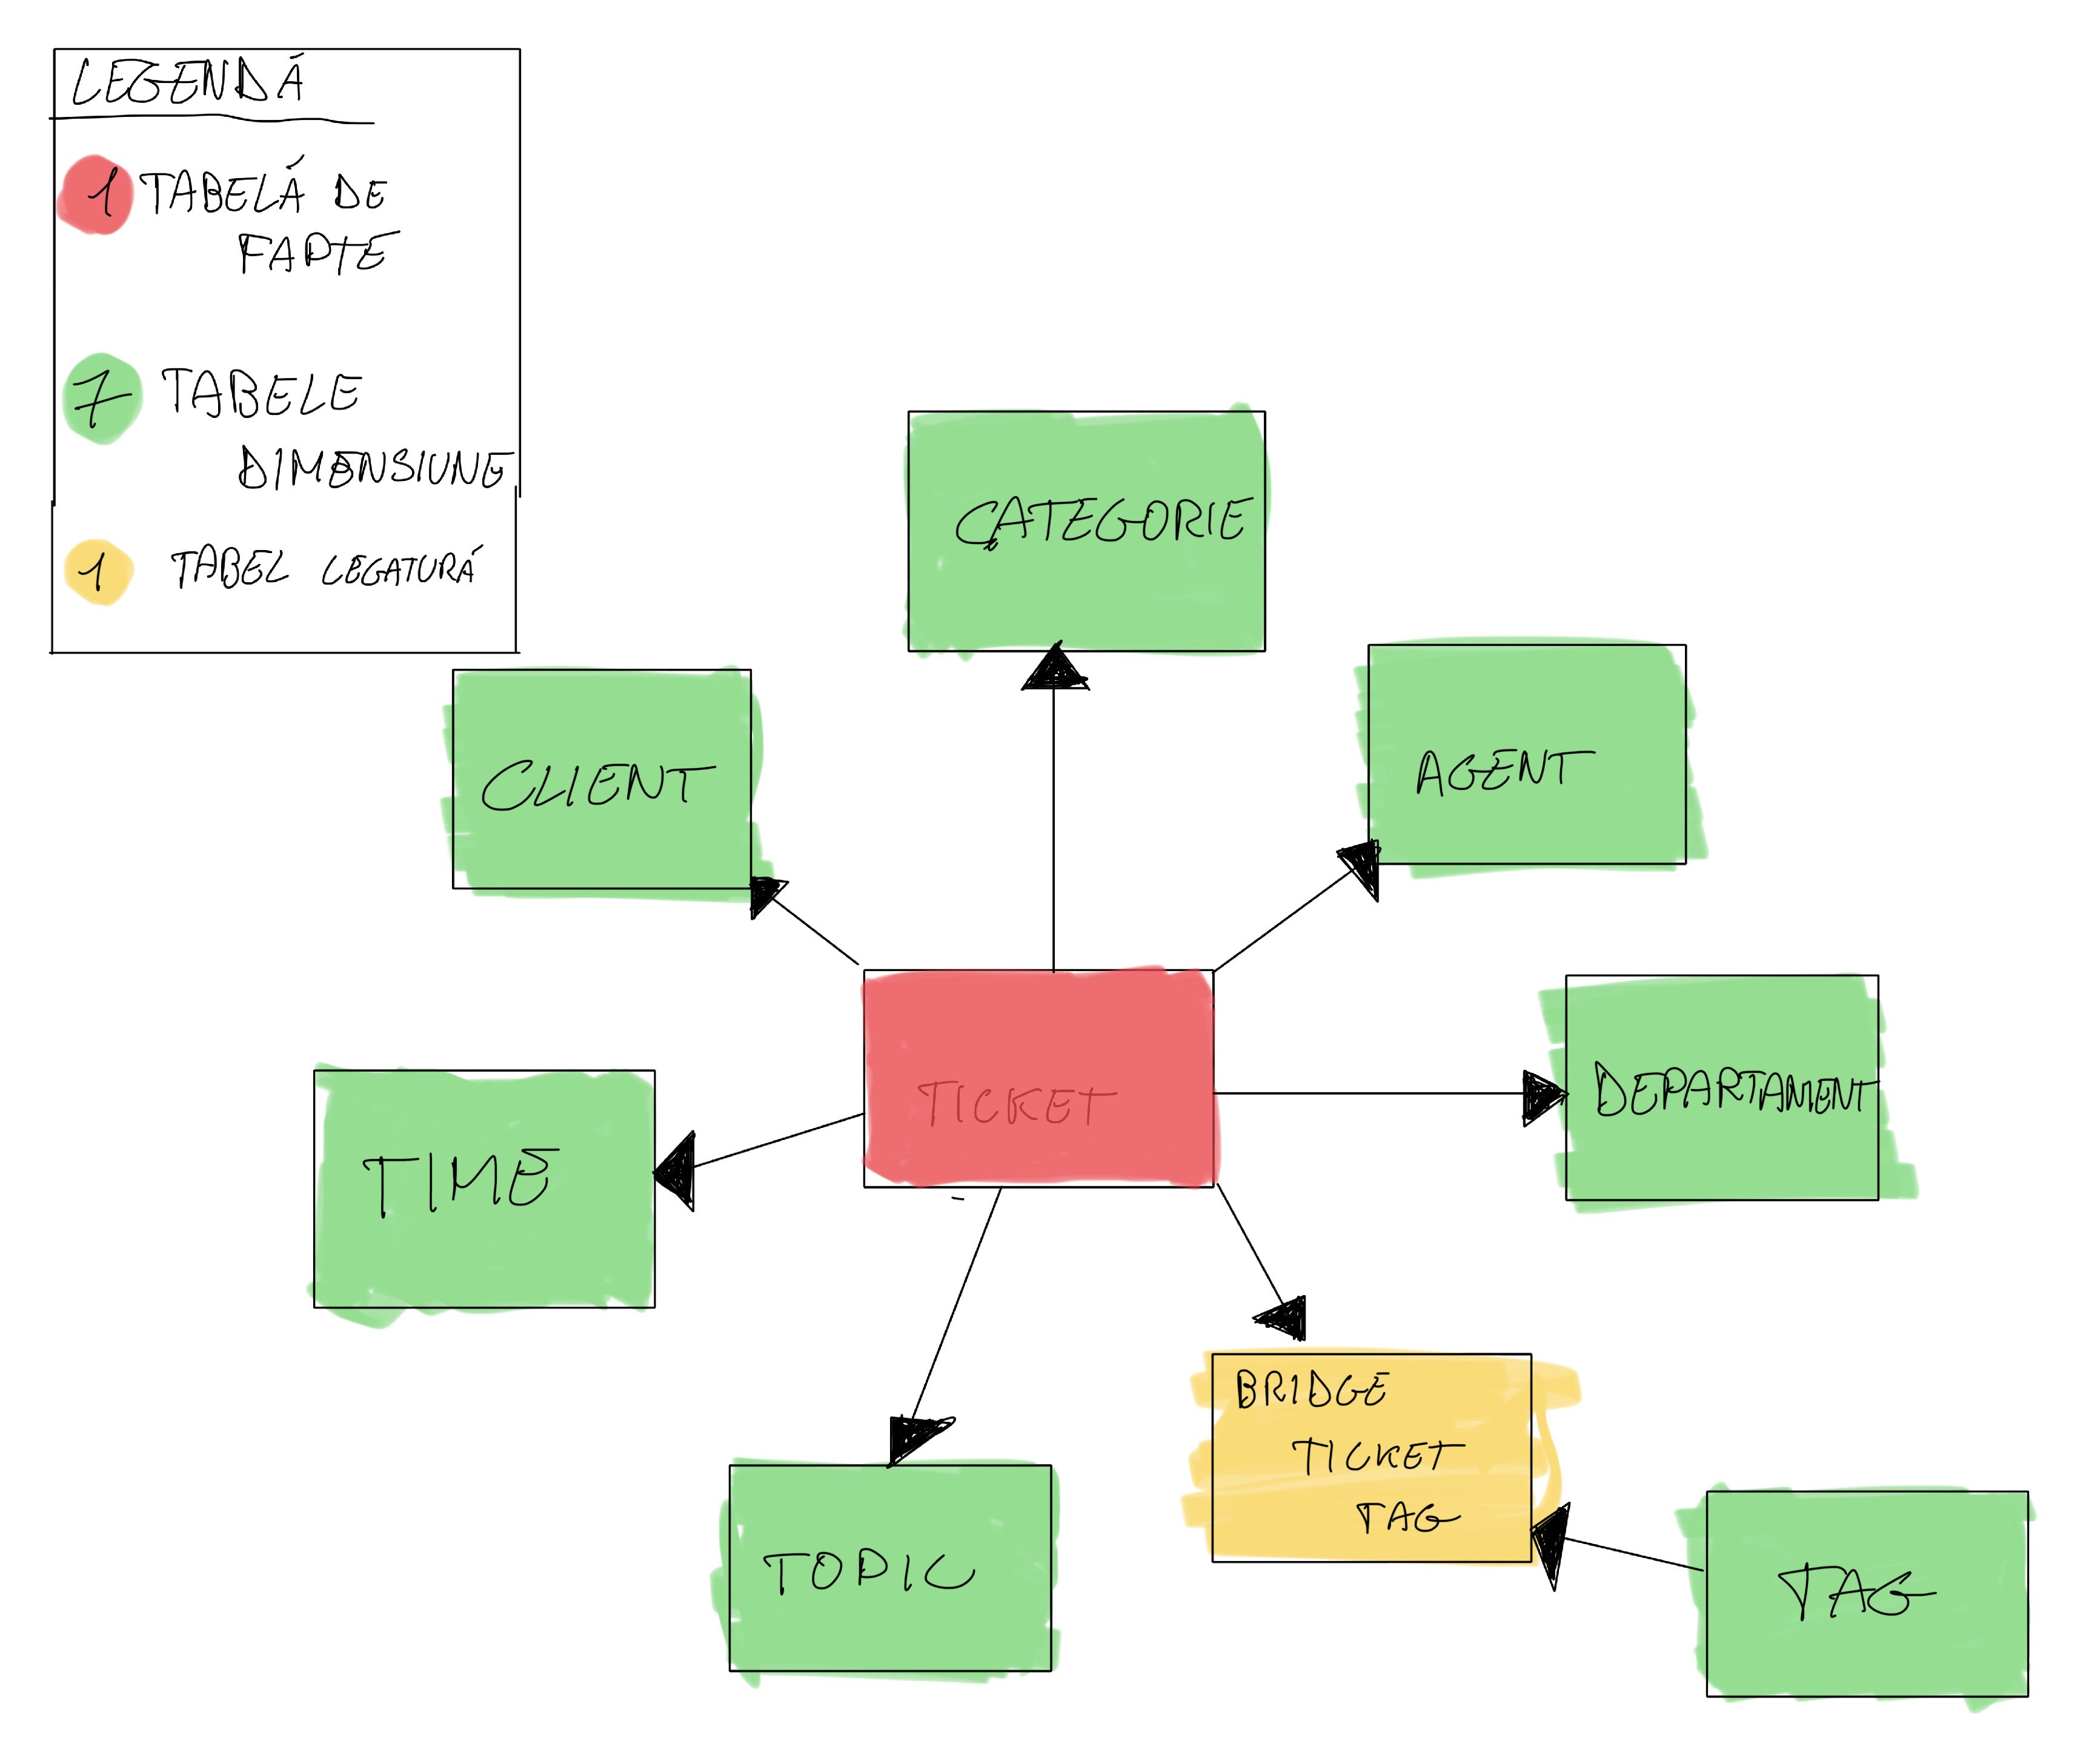
\includegraphics[width=1.0\textwidth]{../../schema/TickLy Schema Stea Simplificata.pdf}
    \caption{Diagrama Stea a Bazei de Date Depozit}
    \label{fig:stea_diagram}
\end{figure}

\section{Structura Modelului Stea}

Modelul stea implementat pentru TickLy conține:

\subsubsection{Tabel de Fapte}

\begin{itemize}
    \item \textbf{FACT\_TICKET} — tabelul central de fapte care stochează măsurile și metricile asociate tichetelor (chei către dimensiuni, status, prioritate, cost estimativ, timp rezolvare)
\end{itemize}

\subsubsection{Tabel de Legătură (Bridge)}

\begin{itemize}
    \item \textbf{BRIDGE\_TICKET\_TAG} — tabel de legătură many-to-many între \texttt{FACT\_TICKET} și \texttt{DIM\_TAG}; permite asocierea mai multor tag-uri la un ticket, cu \texttt{weight\_factor} (ex. 1 / număr tag-uri per ticket)
\end{itemize}

\subsubsection{Tabele Dimensiune}

\begin{enumerate}
    \item \textbf{DIM\_CLIENT} - dimensiunea clienților (Type 2 SCD pentru istoricizare)
    \item \textbf{DIM\_AGENT} - dimensiunea agenților (Type 2 SCD)
    \item \textbf{DIM\_DEPARTAMENT} - dimensiunea departamentelor (Type 2 SCD)
    \item \textbf{DIM\_CATEGORIE} - dimensiunea categoriilor (Type 1 SCD)
    \item \textbf{DIM\_TOPIC} - dimensiunea topic-urilor (Type 1 SCD)
    \item \textbf{DIM\_TAG} - dimensiunea tag-urilor (Type 1 SCD)
    \item \textbf{DIM\_TIME} - dimensiunea temporală pentru analize pe perioade
\end{enumerate}

\begin{itemize}
    \item \textbf{Nota - Type 1 SCD:} nu permite urmărirea istoricului modificărilor.
    \item \textbf{Nota - Type 2 SCD:} permite urmărirea istoricului modificărilor.
\end{itemize}

\section{Caracteristici ale Modelului}

\begin{itemize}
    \item \textbf{Slowly Changing Dimensions (SCD)}: Dimensiunile \texttt{DIM\_CLIENT}, \texttt{DIM\_AGENT} și \texttt{DIM\_DEPARTAMENT} sunt implementate ca Type 2 SCD, permițând urmărirea istoricului modificărilor
    \item \textbf{Degenerări}: Status și Prioritate sunt degenerate în tabelul de fapte (stocate direct în \texttt{FACT\_TICKET})
    \item \textbf{Dimensiune Conformată}: Dimensiunea temporală \texttt{DIM\_TIME}
\end{itemize}
